
\documentclass[preprint,12pt]{elsarticle}
\makeatletter
\def\ps@pprintTitle{%
 \let\@oddhead\@empty
 \let\@evenhead\@empty
 \def\@oddfoot{\centerline{\thepage}}%
 \let\@evenfoot\@oddfoot}
\makeatother

\usepackage[spanish]{babel}
\usepackage{amssymb}
\usepackage{graphicx}
\usepackage{lineno}
\usepackage[utf8]{inputenc}
\usepackage{url}
\usepackage{natbib} 
\usepackage{amsmath} 
\usepackage{amssymb} 

\begin{document}
	\begin{frontmatter}
		\title{\huge Informe de Laboratorio Nro 07}
		\address{Universidad Privada de Tacna}
		\address{Escuela Profesional de Ingeniería de Sistemas}
		\address{Curso : Base de Datos II}		
		\author{Aponte Roldan, Sigfredo        (2016054468)}		
		\address{Tacna, Perú}
	\end{frontmatter}

%% INFORMACIÓN GENERAL -----------------------------------------------------------------------------------------------------------------------------------
\section{INFORMACIÓN GENERAL} 

\subsection {\textbf{Objetivos}}
\begin{itemize}
	\item Despliegue de contenedores.
\end{itemize}

\subsection {\textbf{Equipos, materiales, programas y recursos utilizados}}
\begin{itemize}
	\item Computadora con sistema operativo Windows XP, Vista, Windows 7, Windows 8 y/o Windows 8.1.
	\item Docker Desktop (Para lo cual se debe primero crear una cuenta en Docker Hub)
\end{itemize}

%% MARCO TEORICO -----------------------------------------------------------------------------------------------------------------------------------
\section{MARCO TEÓRICO}
\begin{itemize}
\item Contenedor: Docker trabaja con algo que se llama “contenedores de Linux” estos son un conjunto de tecnologías que juntas forman un contenedor (de Docker).Las herramientas del contenedor, como Docker, ofrecen un modelo de implementación basado en imágenes. Esto permite compartir una aplicación, o un conjunto de servicios, con todas sus dependencias en varios entornos.
\item Docker: Es un proyecto de código abierto que automatiza el despliegue de aplicaciones dentro de contenedores de software, proporcionando una capa adicional de abstracción y automatización de virtualización de aplicaciones en múltiples sistemas operativos.
\end{itemize}

%% PROCEDIMIENTO -----------------------------------------------------------------------------------------------------------------------------------
\section{PROCEDIMIENTO}
\textbf{Paso 1 : Iniciando Docker}
\begin{enumerate}[a)]
\item Hacemos doble clic en el acceso directo "Docker Desktop" para inciar Docker. Luego presionamos clic derecho sobre el icono y seleccionamos la opción "Sig In".
\begin{figure}[htb]
	\begin{center}
		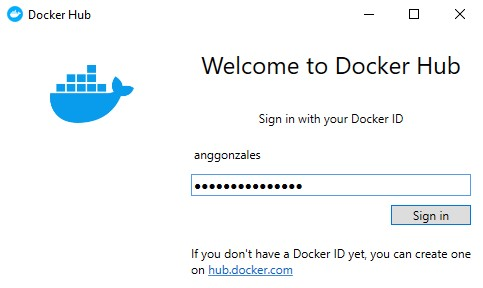
\includegraphics[width=8cm]{./IMAGENES/Docker01}
	\end{center}
\end{figure}
\item Ingresamos nuestras credenciales usuario  y contraseña.
\item Ejecutamos la aplicación PowerShell, ejecutamos como Administrador. En la ventana de comandos digitamos lo siguiente \textbf{docker version}.
\begin{figure}[htb]
	\begin{center}
		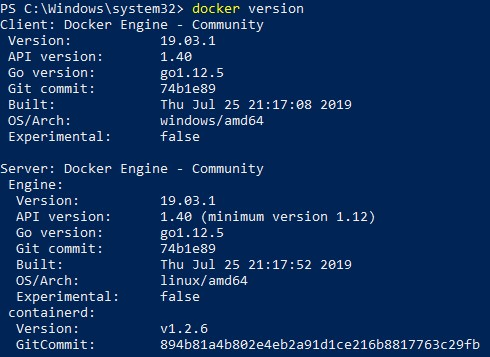
\includegraphics[width=6cm]{./IMAGENES/Docker02}
	\end{center}
\end{figure}


\textbf{Paso 2 : Creando un contenedor con Microsoft SQL Server para Linux}
\item Ejecutamos el siguiente comando \textbf{docker search mssql} en la ventana de PowerShell.
\begin{figure}[htb]
	\begin{center}
		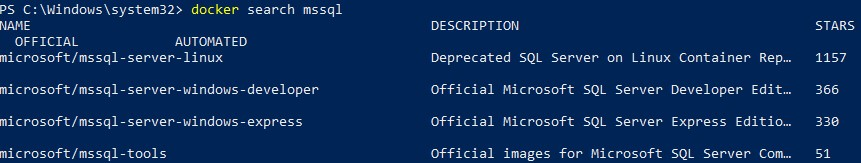
\includegraphics[width=11cm]{./IMAGENES/Docker03}
	\end{center}
\end{figure}
\item Ingresamos a nuestra cuenta en la página web Desktop Hub y buscamos el repositorio \textbf{"microsoft/mssql-server-linux"}. 
\begin{figure}[htb]
	\begin{center}
		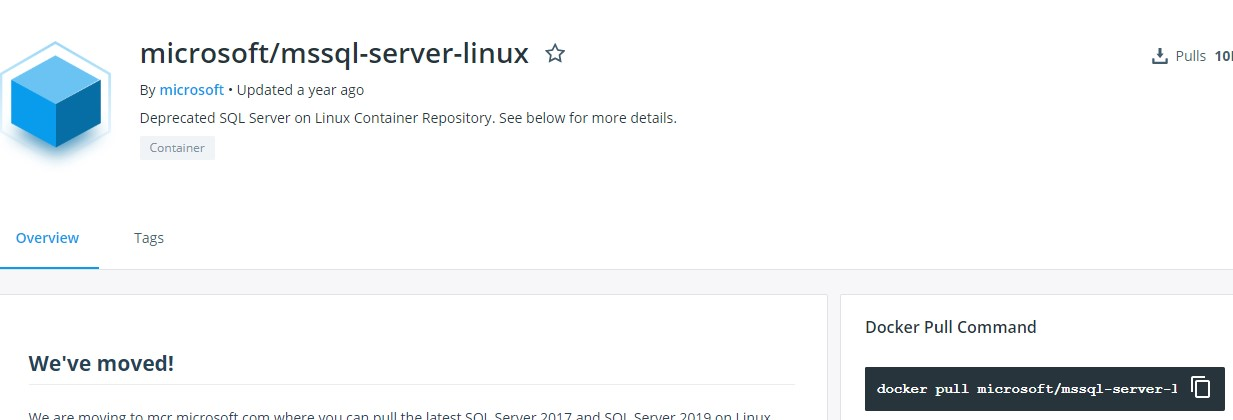
\includegraphics[width=9cm]{./IMAGENES/Docker04}
	\end{center}
\end{figure}
\item Copiamos el comando en la aplicación PowerShell. \begin{center}docker pull microsoft/mssql-server-linux\end{center}
El comando descargará la imagen del contenedor de Microsoft SQL Server en un servidor Linux y mostrará la siguiente resultado.
\begin{figure}[htb]
	\begin{center}
		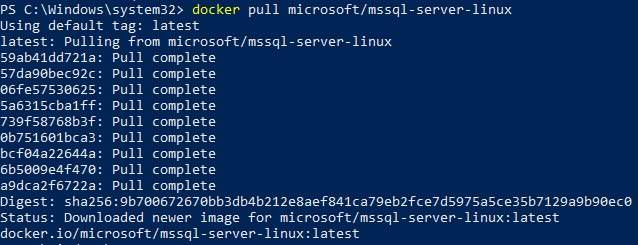
\includegraphics[width=11cm]{./IMAGENES/Docker05}
	\end{center}
\end{figure}


\item Verficamos la imagen con el siguiente comando \textbf{docker images}.
\begin{figure}[htb]
	\begin{center}
		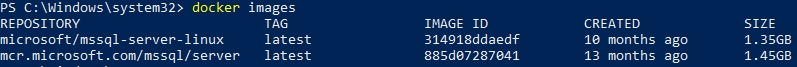
\includegraphics[width=14cm]{./IMAGENES/Docker06}
	\end{center}
\end{figure}

\item Luego digitamos el siguiente comando para iniciar un nuevo contenedor. 
\begin{figure}[htb]
	\begin{center}
		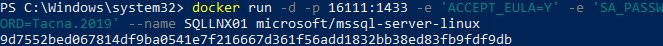
\includegraphics[width=14cm]{./IMAGENES/Docker07}
	\end{center}
\end{figure}

\item La ejecución del comando anteriorr nos delvoverá el ID del contenedor.
\begin{center}
9d7552bed067814df9ba0541e7f216667d361f56add1832bb38ed83fb9fdf9db
\end{center}

\item Verificamos que el contenedor se está ejecutando correctamente con el siguiente comando docker ps. El resultado será similar al siguiente:
\begin{figure}[htb]
	\begin{center}
		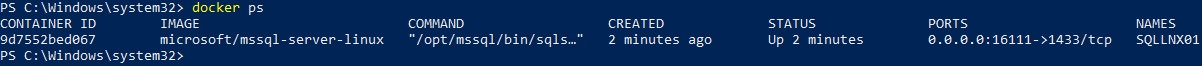
\includegraphics[width=14cm]{./IMAGENES/Docker08}
	\end{center}
\end{figure}

\item Abriremos el programa Microsoft SQL Server Management Studio 17 y conectamos con los siguientes datos: 
\begin{center}Nombre del servidor : 127.0.0.1,16111\end{center}
\begin{center} Inicio de sesión :sa\end{center}
\begin{center}Contraseña: Tacna.2019\end{center}
	\begin{figure}[htb]
		\begin{center}
		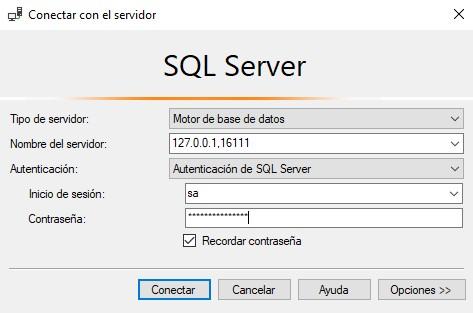
\includegraphics[width=9cm]{./IMAGENES/Docker13}
		\caption{Conectar con el Servidor}
		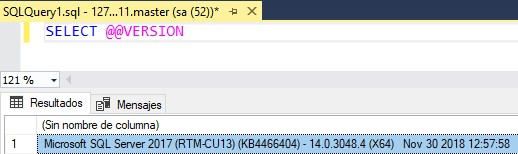
\includegraphics[width=8cm]{./IMAGENES/Docker11}
		\end{center}
	\end{figure}

\item Iniciamos una nueva consulta, escribir y ejecutar la siguiente sentencia:
\begin{center}SELECT @@VERSION\end{center}

\item En la aplicación PowerShell ejecutamos el siguiente comando:
\begin{center}docker rm -f SQLLNX01\end{center}
\item Verificamos la eliminación del contenedor con el siguiente comando:
\begin{center}docker ps\end{center}
\end{enumerate}

%% ANÁLISIS E INTERPRETACIÓN DE RESULTADOS -----------------------------------------------------------------------------------------------------------------------------------
\section{ANÁLISIS E INTERPRETACIÓN DE RESULTADOS}
\begin{enumerate}[a)]
\item Con el comando para iniciar con un contenedor podemos asignar los siguientes parámetros:
\begin{center} -p : 	Asignar el puerto.\end{center}
\begin{center}'sapassword' : Contraseña del Inicio de Sesion SQL, usuario sa.\end{center}
\begin{center} --name : Nombre del contenedor.\end{center}
\end{enumerate}


\section{CUESTIONARIO}

\begin{enumerate}[a)]
\item ¿Con qué comando(s) exportaría la imagen de Docker de Microsoft SQL Server a otra PC o servidor?\newline
Exportar la Imagen de Docker de Microsoft SQL Server
"docker export (ID contenedor) >  Nombreimagen.tar"
\begin{center} docker 9d7552bed067814df9ba0541e7f216667d361f56add1832bb38ed83fb9fdf9db > SQL.tar \end{center}
\begin{figure}[htb]
	\begin{center}
		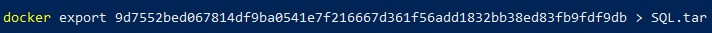
\includegraphics[width=14cm]{./IMAGENES/Docker17}
	\end{center}
\end{figure}
\item ¿Con qué comando(s) podría generar dos volúmenes para un contenedor para distribuir en un volumen el Archivo de Datos (.mdf) y en otro el Archivo Log (.ldf)?\newline
CREATE DATABASE NAMEDATABASE ON \newline
( FILENAME = N'/var/opt/mssql/data2/NDATABASE.mdf' ),\newline
( FILENAME = N'/var/opt/mssql/data2/NDATABASElog.ldf' )\newline
FOR ATTACH\newline
GO\newline
\item Genere un nuevo contenedor y cree la base de datos con las siguientes características.\newline
Nombre : FINANCIERA \newline
Archivos:
\begin{itemize}
\item DATOS (mdf) : Tamaño Inicial : 50MB, Incremento: 10MB, Ilimitado
\item INDICES (ndf) Tamaño Inicial : 100MB, Incremento: 20MB, Maximo: 1GB
\item HISTORICO (ndf) Tamaño Inicial : 100MB, Incremento: 50MB, Ilimitado
\item LOG (ldf) Tamaño Inicial : 10MB, Incremento: 10MB, Ilimitado
\end{itemize}
\item ¿Cuál sería el script SQL que generaría esta base de datos?
\begin{figure}[htb]
	\begin{center}
		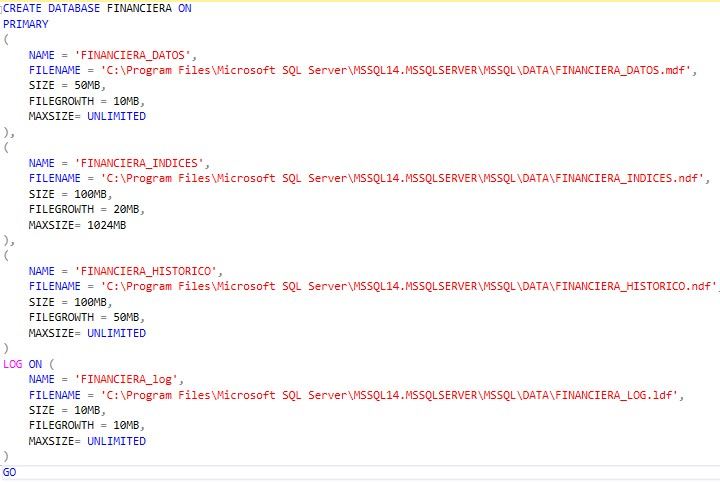
\includegraphics[width=10cm]{./IMAGENES/Docker14}
		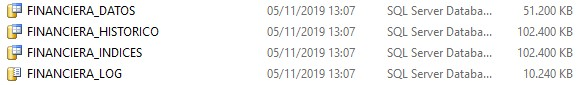
\includegraphics[width=10cm]{./IMAGENES/Docker15}
	\end{center}
\end{figure}
\end{enumerate}



\section{CONCLUSIONES}
La perspectiva de Docker de empaquetado liviano e implementación de aplicaciones y dependencias es emocionante, y la comunidad la está adoptando rápidamente.
y se está abriendo camino en entornos de producción. Por ejemplo, Red Hat anunció en diciembre soporte para Docker en el próximo Red Hat Enterprise Linux 7.
Sin embargo, Docker sigue siendo un proyecto joven y está creciendo a una velocidad vertiginosa. Será emocionante ver cómo el proyecto se acerca a su versión 1.0, que se supone sera la primera versión oficialmente sancionada para entornos de producción. Docker se basa en tecnologías establecidas, algunas de las cuales han existido durante más de un década, pero eso no lo hace menos revolucionario. Esperemos que este artículo proporcione suficiente información e inspiración para descargar Docker y experimentar con la herramienta.

\section{WEBGRAFIA}
https://es.wikipedia.org/wiki/Docker(software)\newline
https://docs.docker.com/get-started/\newline
https://www.redhat.com/es/topics/containers/what-is-docker\newline
\end{document}
